\documentclass{resume}

\begin{document}

\fontfamily{ppl}\selectfont

\noindent
\begin{tabularx}{\linewidth}{@{}m{0.8\textwidth} m{0.2\textwidth}@{}}
{
    \Large{John Doe} \newline
    \small{
        \clink{
            \href{mailto:johndoe@mailme.com}{johndoe@mailme.com} \textbf{·} 
            {\fontdimen2\font=0.75ex +1 2345 6789} 
            \textbf{·} 
            \href{https://johnmyweb.com}{johnmyweb.com}
        } \newline
        New York, USA
    }
} & 
{
    \hfill
    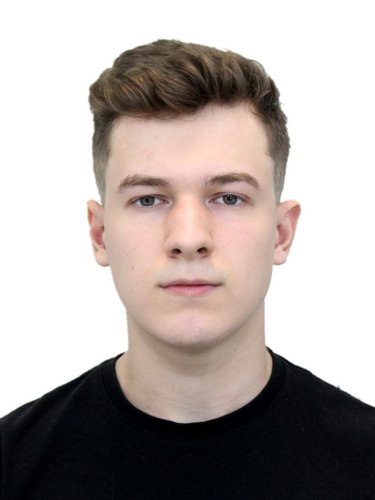
\includegraphics[width=2.8cm]{images/gr.png}
}
\end{tabularx}
\begin{center}
\begin{tabularx}{\linewidth}{@{}*{2}{X}@{}}
% left side %
{
    \csection{EXPERIENCE}{\small
        \begin{itemize}
            % item 1 %
            \item \frcontent{Dream Company}{Senior Software Engineer - San Fransisco, CA}{Co-designer and co-implementor of five successive generations of Google’s crawling indexing and query retrieval systems.}{August 1999 onwards}
            % item 2 %
            \item \frcontent{Old Dream Company}{Senior Member of Technical Staff − Texas}{Designer and implementor of a system for retrieving and caching electronic commerce content including a crawler and custom full-text indexing system that allows flexible keyword searching of product information.}{February 1999 to August 1999}
        \end{itemize}
    }
    \csection{EDUCATION}{\small
        \begin{itemize}
            % item 1 %
            \item \frcontent{Ph.D. Computer Science}{University of Washington}{}{1996}
            \item \frcontent{B.S. Computer Engineering, CGPA: 3.6/4}{University of Minnesota}{}{1990}
        \end{itemize}
    }
    \csection{AWARDS \& RECOGNITION}{\small
        \begin{itemize}
            % item 1 %
            \item \frcontent{Fake Academy Fellow}{Fake Academy of Arts and Sciences}{}{2016}
            % item 2 %
            \item \frcontent{Elon Musk Award}{State of Engineering}{}{2012}
            % item 3 %
            \item \frcontent{ACM Fellow}{Association for Computing Machinery}{}{2009}
        \end{itemize}
    }
} 
% end left side %
& 
% right side %
{
    \csection{SKILLS}{\small
        \begin{itemize}
            \item \textbf{Technologies} \newline
            {\footnotesize Golang, Python, C++, Tensorflow, Spanner, Bigtable, MapReduce, Google Cloud Platform,  Protocol Buffers}{}{}
            \item \textbf{Patterns \& Practices} \newline
            {\footnotesize Object Oriented Programming, Functional  Programming, CI \& CD, Microservices}
            \item \textbf{Project Management} \newline
            {\footnotesize Agile, Scrum, Google Bug Tracker, Google Workspace}
        \end{itemize}
    }
    \csection{PROJECTS}{\small
        \begin{itemize}
            \item \frcontent{Tensorflow \clink{\href{https://tensorflow.org}{[tensorflow.org]}}}{An open-source machine-learning software library}{}{C++, Python, Bash}
            \item \frcontent{LevelDB \clink{\href{http://github.com/google/leveldb}{[github.com/google/leveldb]}}}{An open-source on-disk key-value store}{}{C++}
            \item \frcontent{Spanner \clink{\href{http://google.com/spanner}{[google.com/spanner]}}}{A scalable, multi-version, globally distributed, and synchronously replicated database}{}{C++, Java, Bash}
        \end{itemize}
    }
    \csection{OTHER HIGHLIGHTS}{\small
        \begin{itemize}
            \item {\footnotesize Gave talk on \textit{Achieving Rapid Response Times in Large Online Services} at Berkeley AMPLab Cloud.}
            \item {\footnotesize Led several teams across infrastructure, founded \textit{Google Brain} and was involved in hiring process.}
        \end{itemize}
    }
    \csection{HOBBIES \& INTERESTS}{\small
        \vspace{0.32cm}
        \begin{tabularx}{\linewidth}{@{}*{4}{>{\centering\arraybackslash}X}@{}}
            {\centering
            
\includegraphics[width=0.8cm]{images/userexperience.png}
            } &
            {\centering
            
\includegraphics[width=0.8cm]{images/lamp.png}
            } & 
            {\centering
            
\includegraphics[width=0.8cm]{images/healthcare.png}
            } &
            {\centering
            
\includegraphics[width=0.8cm]{images/cauldron.png}
            } \\
            {\footnotesize UI/UX} & {\footnotesize Problem Solving} & {\footnotesize Healthcare} & {\footnotesize Open Source}
        \end{tabularx}
    }
}
\end{tabularx}
\end{center}
\end{document}